\documentclass[10pt, a4paper]{article}
\usepackage[utf8]{inputenc}
\usepackage[margin=0.5in]{geometry}
\usepackage[portuguese]{babel}
\usepackage{graphicx}
\usepackage{amsmath}

\setlength{\parindent}{0pt}
\graphicspath{ {./images/} }

\title{Sinais e Sistemas - Trabalho 2}
\author{
    Leonardo Soares da Costa Tanaka\\
    Matheus Henrique Sant Anna Cardoso \\
    Theo Rudra Macedo e Silva
}
\date{Setembro de 2022}

\begin{document}

\maketitle

%% Primeira questao
{\textbf 1.)} Uma nota musical, ou tom, pode ser modelada por um sinal periódico com uma frequência fundamental e vários harmônicos. Quando duas notas musicais são “tocadas” ao mesmo tempo — um acorde — o efeito resultante pode soar agradável, consonante ou desagradável, dissonante. Desde os antigos gregos, com Pitágoras, se sabe que as combinações ou acordes agradáveis acontecem quando a razão entre as frequências fundamentais das notas é expressa por números naturais pequenos. Assim, os acordes mais harmônicos e consonantes são, pela ordem, aqueles associados às razões 1:1 (uníssono), 2:1 (oitava), 3:2 (5.a perfeita), 4:3 (4.a perfeita), 5:4 (3.a maior) etc.\\
(a) Crie, no Octave, uma nota com frequência \textbf{G2:} $f_{0} = 170Hz$, usando ondas quadradas ou triangulares (pesquise e use os comandos {\texttt square} ou {\texttt sawtooth} no Octave) em uma escala de tempo de 3 segundos com espaçamento entre as amostras de {\texttt{dt = 1/44000 (t=0:dt:3)}} e chame-a de tônica $x_{t}(t)$;\\
(b) crie a oitava $x_{8}(t)$ da tônica, a 5.a $x_{5}(t)$, a 4.a $x_{4}(t)$, a 2.a (9:8) $x_{2}(t)$ e também a nota com relação 321:319 $x_{d}(t)$;\\
(c) usando o comando {\texttt sound(x, 44000)} ouça no Octave as notas isoladas e todos os acordes (para os acordes, crie a soma {\texttt{z = xt + x8}}, por exemplo, e depois use o comando {\texttt sound} acima em z) verificando se são consonantes;\\
(d) explique a teoria harmônica de Pitágoras usando Série de Fourier e análise dos harmônicos da tônica e das companheiras.

\vspace{\baselineskip}
%% Segunda questao
{\textbf 2.)} Um sinal definido como abaixo em um intervalo de largura $L = 4$ e nulo para outros valores de $t$ é chamado de pulso:\\
{\textbf G2:} $x(t) = 1 - e^{|t|}$ para $- L/2 \leq t < L/2$\\
{\textbf{(a)}} Esboce o gráfico do pulso;

\begin{figure}[h]
    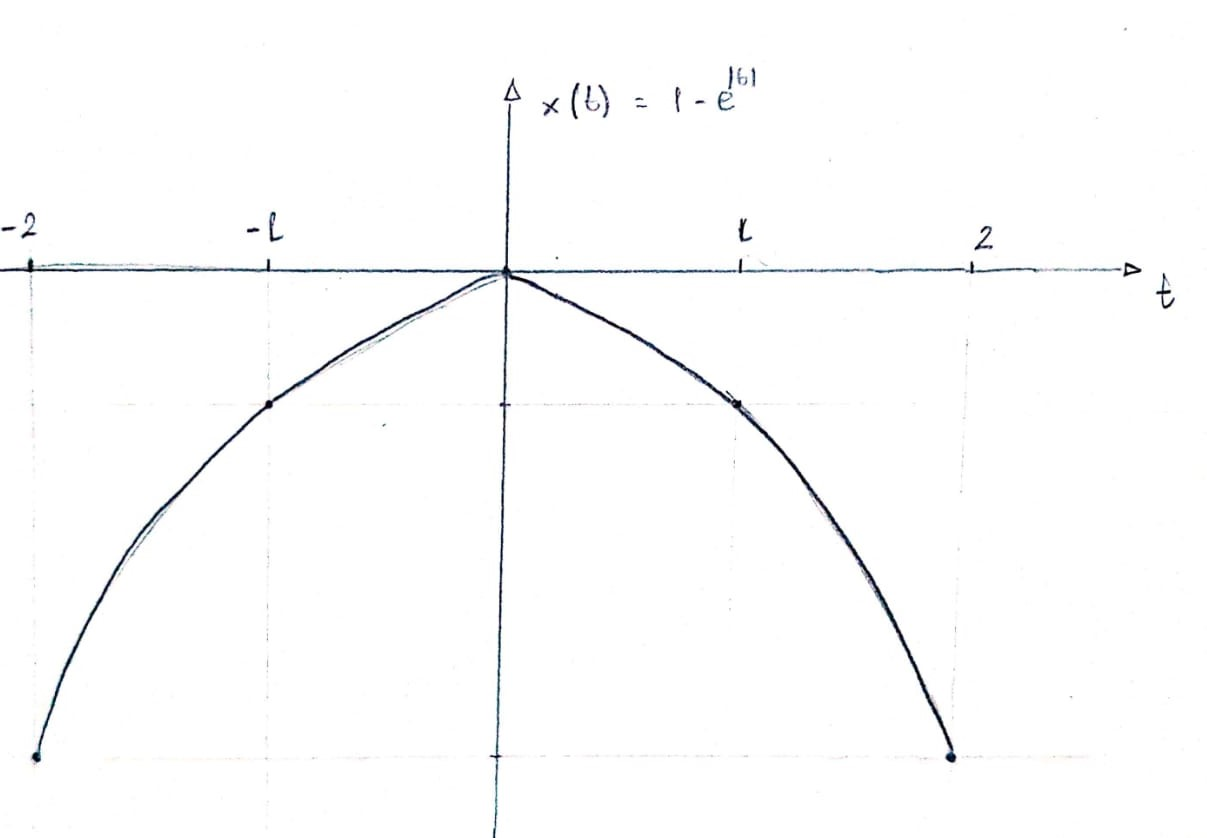
\includegraphics[scale=0.3]{plot2a.jpeg}
    \centering
\end{figure}

{\textbf{(b)}} calcule sua energia total $E_{t}$;\\
O que buscamos é:
\[E_{t} = \int_{-2}^{2} |1 - e^{|t|}|^2\,dt\]
Para motivações de cálculo, podemos separar esta integral em duas partes:
\[E_{t} = \int_{-2}^{0} (1 - e^{-t})^{2}\,dt + \int_{0}^{2} (1 - e^{t})^{2}\,dt\]
Porém, como o gráfico possui eixo de simetria em $t = 0$, sabemos que o valor das duas integrais separadas é igual. Dessa forma fazemos:
\[E_{t} = 2 \cdot \int_{-2}^{0} (1 - e^{-t})^{2}\,dt = 2 \cdot \int_{0}^{2} (1 - e^{t})^{2}\,dt\]
Escolhendo a que melhor convém para o cálculo, obtemos:
\[E_{t} = 2 \cdot \int_{0}^{2} (1 - e^{t})^{2}\,dt\]
Finalmente:
\[E_{t} = 2 \cdot \int_{0}^{2} (1 - 2e^t + e^{2t})\,dt\]
\[E_{t} = 2 \cdot \bigl[t - 2e^t + e^{2t} \bigr]_{0}^{2}\]
\[E_{t} = 7 - 4e^2 + e^{4}\]
Fazendo os cálculos utilizando o Octave, a energia total será:
\[E_{t} = 32.042\]

{\textbf{(c)}} calcule $X(0)$ fazendo $f = 0$ na fórmula de definição;\\
Primeiramente, anotemos a definição com a fórmula abaixo:
\[X(f) = \int_{-\infty}^{\infty} x(t) e^{-j2\pi ft}\,dt\]
Deve-se perceber que o intervalo de integração será de $[-2\,2]$.
Como queremos $X(0)$, fazemos $f = 0$ na fórmula:
\[X(0) = \int_{-2}^{2} x(t) e^{-j2\pi 0t}\,dt\]
\[X(0) = \int_{-2}^{2} (1 - e^{|t|})\,dt\]
Separando, novamente, em duas integrais, temos:
\[X(0) = \int_{-2}^{0} (1 - e^{-t})\,dt + \int_{0}^{2} (1 - e^{t})\,dt\]
\[X(0) = (t + e^{-t})\bigg|_{-2}^{0} + (t - e^{t})\bigg|_{0}^{2}\]
\[X(0) = 3 - e^2 + 3 - e^2\]
\[X(0) = 6 - 2e^2\]

\vspace{\baselineskip}

{\textbf{(d)}} calcule analiticamente $X(f)$ e verifique se $X(0)$ pode ser obtido a partir desta fórmula sem indeterminações;\\
Agora, queremos calcular a seguinte integral:
\[X(f) = \int_{-2}^{2} (1 - e^{|t|})e^{-j2\pi ft}\,dt\]
Aqui, podemos, novamente, separar em duas integrais:
\[X(f) = \int_{-2}^{0} (1 - e^{-t})e^{-j2\pi ft}\,dt + \int_{0}^{2} (1 - e^{t})e^{-j2\pi ft}\,dt\]
\[X(f) = \biggl(-\frac{e^{-j2\pi ft}}{j2\pi f} + \frac{e^{-t(1 + j2\pi f)}}{1 + j2\pi f}\biggr)\bigg|_{-2}^{0} + 
\biggl(-\frac{e^{-j2\pi ft}}{j2\pi f} - \frac{e^{t(1 - j2\pi f)}}{1 - j2\pi f}\biggr)\bigg|_{0}^{2}\]
\[X(f) = -\frac{1}{j2\pi f} + \frac{1}{1 + j2\pi f} + \frac{e^{j4\pi f}}{j2\pi f} - \frac{e^2e^{j4\pi f}}{1 + j2\pi f} +
\frac{1}{j2\pi f} + \frac{1}{1 - j2\pi f} - \frac{e^{-j4\pi f}}{j2\pi f} - \frac{e^2e^{-j4\pi f}}{1 - j2\pi f}\]
Resumindo as contas, temos:
\[X(f) = 4sinc(4f) + \frac{2}{1 + 4\pi^2f^2} - \frac{2e^2cos(4\pi f)}{1 + 4\pi^2 f^2} - \frac{4e^2\pi f sen(4\pi f)}{1 + 4\pi^2 f^2}\]
Primeiramente, perceba que os valores de $X(f)$ são reais.\\
Agora, que temos a expressão, calculemos $X(0)$ com base nela e comparar com a expressão obtida em (c).
\[X(0) = 4sinc(0) + \frac{2}{1 + 4\pi^2 0} - \frac{2e^2cos(4\pi 0)}{1 + 4\pi^2 0} - \frac{4e^2\pi 0 sen(4\pi 0)}{1 + 4\pi^2 0}\]
\[X(0) = 4 + 2 - 2e^2 = 6 - 2e^2\]
Perceba, então, que obtivemos a mesma expressão, não existindo indeterminações para $f = 0$.

\vspace{\baselineskip}

{\textbf{(e)}} trace o espectro de energia $|X(f)|^{2} \times f$ para $f \in [-1\,+ 1]Hz$ usando muitos pontos e calcule a energia contida nesta banda $(\int_{-1}^{1} |X(f)|^{2}\,dt)$ usando integração aproximada;\\
Utilizando o Octave para calcular a aproximação do espectro de energia e plotar o gráfico. O resultado é o visto abaixo:

\begin{figure}[h]
    \begin{minipage}[!]{0.50\linewidth}
        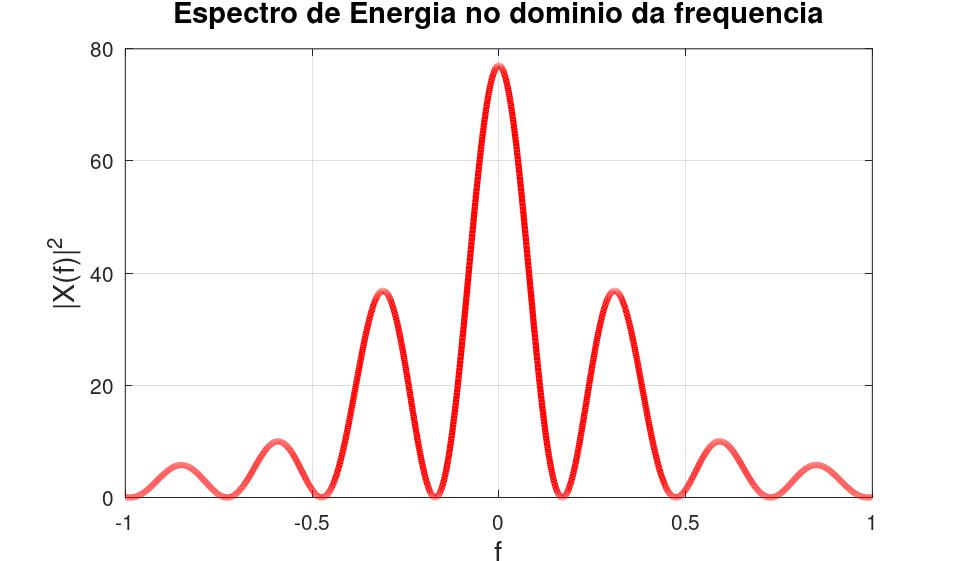
\includegraphics[scale=0.27]{plot2e.jpg}        
    \end{minipage}
    \begin{minipage}[!]{0.48\linewidth}
        Calculando a energia para o intervalo definido (de -1 até 1), utilizando o próprio Octave para realizar os cálculos aproximados, encontramos que a energia para este intervalo de frequências.
        \[E_{[-1\,1]} = 27.923\]        
    \end{minipage}
\end{figure}

\newpage

{\textbf{(f)}} por tentativa e erro, e usando o método anterior, calcule a banda de passagem que retém $95\%$ da energia do sinal: $f_{M}$ tal que $\int_{-f_{M}}^{f_{M}} |X(f)|^{2}\,df$;

Utilizando, novamente, o software Octave, pudemos testar, para algumas faixas de frequências, quantos porcento da energia havia naquela banda de frequência. O valor mais próximo que chegamos para a frequência $f_{M}$ foi de $2.5985$, em que chegamos a uma retenção de $95.000\%$.
\[E_{t} = 32.042\]
\[E_{f_{M}} = 30.440\]
Finalmente, a banda de passagem que retém $95\%$ da energia é para $f_{M} = 2.5985$.

\vspace{\baselineskip}

%% Terceira questao
{\textbf 3.)} Um sinal é caracterizado por\\
{\textbf G2:} $ X_{m}(f) = 80p_{20}(f + 810) + 80p_{20}(f - 790) $\\
com frequências medidas em $kHz$. Lembrar que $p_{\Delta}(f - \tau)$ denota um pulso de largura $\Delta$, amplitude $\Delta^{-1}$ e aplicado a partir de $\tau$, com transformada conhecida.\\
{\textbf{(a)}} Esboçar os espectros de amplitude e de energia;

\begin{figure}[h]
    \begin{minipage}[!]{0.50\linewidth}
        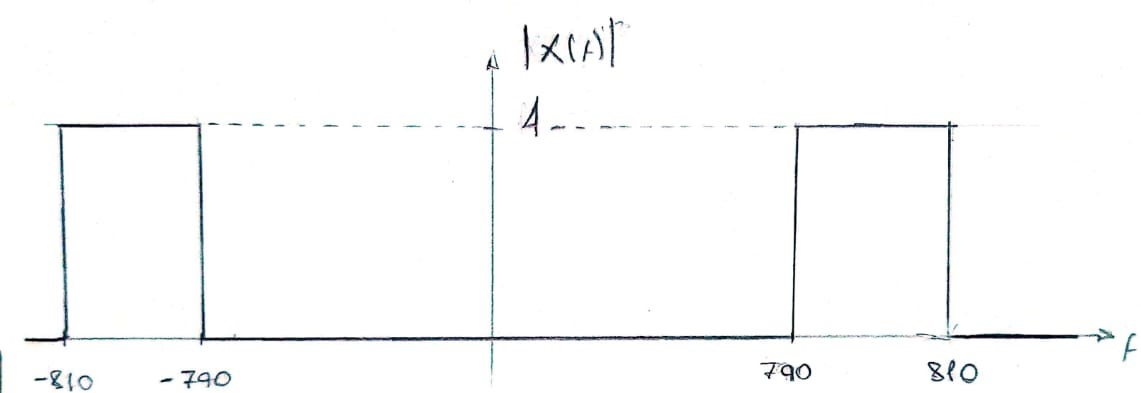
\includegraphics[scale=0.27]{plot3a2.jpeg}
    \end{minipage}
    \begin{minipage}[!]{0.48\linewidth}
        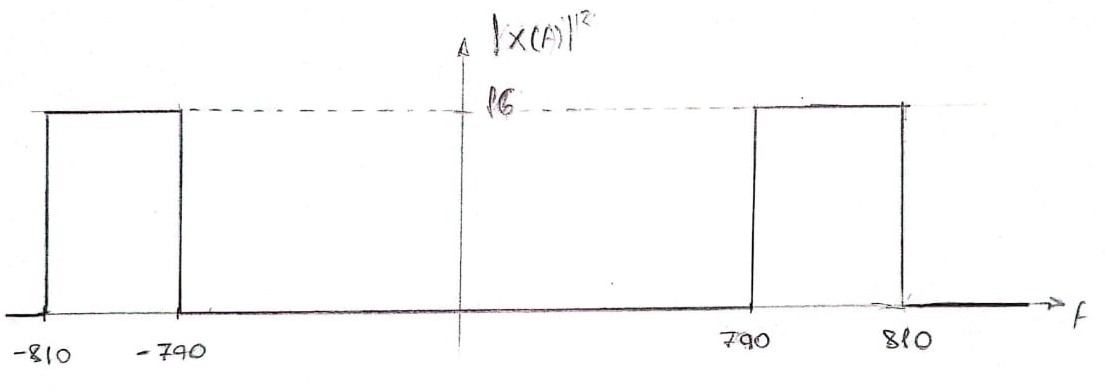
\includegraphics[scale=0.27]{plot3a1.jpeg}
    \end{minipage}
\end{figure}

{\textbf{(b)}} calcular sua anti-transformada de Fourier: $\mathcal{F}^{-1} \{X_{m}(f)\} = x_{m}(t)$ (use as propriedades);

Queremos calcular a inversa da transformada de Fourier. Para isso, usamos:

\[x_{m}(t) = \int_{-810}^{-790} 4e^{j2\pi ft}\,df + \int_{790}^{810} 4e^{j2\pi ft}\, df\]
\[x_{m}(t) = \biggl[\frac{4e^{j2\pi ft}}{j2\pi t}\biggr]_{-810}^{-790} + \biggl[\frac{4e^{j2\pi ft}}{j2\pi t}\biggr]_{790}^{810}\]
\[x_{m}(t) = 4\biggl[\frac{2sen(2\pi 810t)}{2\pi t} - \frac{2sen(2\pi 790t)}{2\pi t}\biggr]\]
\[x_{m}(t) = 4\biggl[\frac{2sen(2\pi 810t) \cdot 810}{2\pi t \cdot 810} - \frac{2sen(2\pi 790t) \cdot 790}{2\pi t \cdot 790}\biggr]\]
\[x_{m}(t) = 6480\,sinc(1620t) - 6320\,sinc(1580t)\]

{\textbf{(c)}} ao sinal $x_{m}(t)$ se aplica um filtro PB (passa-baixas) ideal; determinar sua frequência de corte $M$ de modo que 50\% da energia total seja retida;

Aqui é bem mais conveniente trabalharmos com o sinal no domínio da frequência (o dado da questão), sendo, dessa forma, fácil ver que a frequência de corte assume, nesse caso, o valor de $800Hz$, percorrendo o intervalo de $[-800\, 800]$. Isso fica claro, pois, ao obtermos o espectro de energia, para termos metade do gráfico preenchido (50\% da área), devemos percorrer os valores entre -800 até 800.

\vspace{\baselineskip}

{\textbf{(d)}} ao sinal $x_{m}(t)$ se aplica um filtro PA (passa-altas) ideal; determinar sua frequência de corte $M$ de modo que 50\% da energia total seja retida.

Perceba que, de forma análoga ao anterior, é mais conveniente trabalharmos no domínio da frequência. Aqui, diferentemente, queremos um filtro passa-alta, sendo a frequência de corte, também $800Hz$. Finalmente, obtemos 50\% da área do gráfico de espectro de energia, com os intervalos $[-\infty\,\,-800]$ e $[800\,\,\infty]$. Logo, a frequência de corte é, novamente $800Hz$.

\end{document}